%%% Local Variables:
%%% mode: Xelatex
%%% TeX-master: t
%%% End:
\raggedbottom
\documentclass[draftformat,mathCMR]{WUSTthesis}%草稿用这个
%\documentclass[finalformat,mathCMR]{WUSTthesis}%盲审用这个
%\raggedbottom

\usepackage{WUSTtils}% 所有其它可能用到的包都统一放到这里了,可以根据自己的实际添加或者删除。这样做主要是为了避免class文件过于臃肿。
%\usepackage[a4paper, margin=3.05cm]{geometry}
%\usepackage{mathfont}
\usepackage{amsmath,amssymb,amsfonts,bm}
\usepackage{listings}
\definecolor{codegreen}{rgb}{0,0.6,0}
\definecolor{codegray}{rgb}{0.5,0.5,0.5}
\definecolor{codepurple}{rgb}{0.58,0,0.82}
\definecolor{backcolour}{RGB}{245,245,245}

\lstdefinestyle{mystyle}{
    backgroundcolor=\color{backcolour},   
    commentstyle=\color{codegreen},
    keywordstyle=\color{magenta},
    numberstyle=\tiny\color{codegray},
    stringstyle=\color{codepurple},
    basicstyle=\ttfamily\footnotesize,
    breakatwhitespace=false,         
    breaklines=true,              
    captionpos=b,                    
    keepspaces=true,                 
    numbers=left,                    
    numbersep=5pt,                  
    showspaces=false,                
    showstringspaces=false,
    showtabs=false,                  
    tabsize=2
}
\lstset{style=mystyle, escapeinside=``}
%\usepackage{mathalpha}  % 提供更灵活的字体支持
%\DeclareMathAlphabet{\mathtt}{T1}{pcr}{m}{n}  % 强制关联 Courier New
\usepackage{graphicx}
\usepackage{ragged2e}
\newcolumntype{P}[1]{>{\RaggedRight\hspace{0pt}}p{#1}}
\newcolumntype{Z}{>{\centering\arraybackslash}X}
\usepackage{tabularx}
\usepackage{multirow}
\usepackage{newtxmath}
\DeclareSymbolFont{orilargesymbols}{OMX}{cmex}{m}{n}
\DeclareMathSymbol{\orisum}{\mathop}{orilargesymbols}{"50}
\renewcommand\sum\orisum
\renewcommand\geq\geqslant 
\renewcommand\leq\leqslant  
\RequirePackage[top=3cm, bottom=3cm, left=3cm, right=3cm, headheight=2.0cm, footskip=2.4cm,]{geometry}
\usepackage[font={small, stretch=1.5}, labelfont=bf, textfont=bf]{bicaption}
\captionsetup{labelsep=space}
\captionsetup[figure][bi-first]{name=图, font={small, stretch=1.5}, labelfont=bf, textfont=bf, justification=centering}
\captionsetup[figure][bi-second]{name=Figure, font={small, stretch=1.5}, labelfont=bf, textfont=bf, justification=centering}
\captionsetup[table][bi-first]{name=表, font={small, stretch=1.5}, labelfont=bf, textfont=bf, justification=centering}
\captionsetup[table][bi-second]{name=Table, font={small, stretch=1.5}, labelfont=bf, textfont=bf, justification=centering}
\usepackage[cal=cm]{mathalpha}
%\setmainfont{Times New Roman}[Scale=.9]
\setmainfont{Times New Roman}
%\includeonly{body/chap02}
\PassOptionsToPackage{no-math}{fontspec}
\usepackage{setspace}

\begin{document}
\begin{sloppypar}
%定义所有的eps文件在 figures 子目录下
\graphicspath{{figures/}}

% 生成封面,版权页,摘要

\frontmatter

%%% Local Variables:
%%% mode: Xelatex
%%% TeX-master: t
%%% End:

\ctitle{论文题目}
\iffalse
\xuehao{202102601035} \schoolcode{10488}
\csubjectname{材料科学与工程} \cauthorname{张万成}
\csupervisorname{卢志红} \csupervisortitle{教授}
\defencedate{2025~年~8~月~25~日} \grantdate{}
\chair{}%
\firstreviewer{} \secondreviewer{} \thirdreviewer{}

\etitle{Theoretical Study on Modulation of Altermagnetism and Spin Transport Properties in Rutile Oxides}
\edegree{Doctor of Philosophy in Engineering}
\esubject{Materials Science and Engineering}
\eauthor{Zhang Wancheng}
\esupervisor{Prof. Lu Zhihong}
\fi
\xuehao{} \schoolcode{10488}
\csubjectname{仿宋\_GB2312三号加粗靠下居中} \cauthorname{仿宋\_GB2312三号加粗靠下居中}
\csupervisorname{仿宋\_GB2312三号加粗靠下居中} \csupervisortitle{}
\defencedate{仿宋\_GB2312三号加粗靠下居中} \grantdate{}
\chair{}%
\firstreviewer{} \secondreviewer{} \thirdreviewer{}

\etitle{English Title}
\edegree{Doctor of Philosophy in Engineering}
\esubject{Times New Roman(三号加粗靠下居中)}
\eauthor{Times New Roman(三号加粗靠下居中)}
\esupervisor{Times New Roman(三号加粗靠下居中)}

%定义中英文摘要和关键字
\cabstract{
摘要应具有独立性和自含性,简短明了。博士学位论文摘要1000字左右。关键词是用以表示全文主题内容信息款目的单词或术语(3-5个),关键词之间用“;”隔开。
\textcolor{red}{(宋体、Times New Roman,小四号,1.5倍行距)}
}

\ckeywords{关键词1;关键词2;……;关键词5}



\eabstract{
Externally pressurized gas bearing has been widely used in the field of aviation, semiconductor, weave, and measurement apparatus because of its advantage of high accuracy, 
little friction, low heat distortion, long life-span, and no pollution. In this thesis, based on the domestic and overseas researching……
\textcolor{red}{(Times New Roman小四号,1.5倍行距,首行缩进2个英文字符)}
}
\ekeywords{keyword 1; keyword 2; ……; keyword 5}



\makecover

% 手动设置页码延续
%\pagenumbering{Roman} % 强制大写罗马数字
%\setcounter{page}{2} % 假设摘要结束于Ⅱ,目录从Ⅲ开始

% 生成目录
\clearpage
\pagestyle{tocpage} % 所有后续页使用 tocpage 样式
\thispagestyle{tocpage} % 强制当前页(目录第一页)生效
\tableofcontents
%\tableofengcontents 
\clearpage

% 对照表
%\begin{denotation}
\item[xue] 我的姓
\item[ruini] 我的名
\item[W.M. Zheng]  我的老师
\item[Tsinghua] 学校名
\item[Long] 来个比较长的,看看会出现什么情况。
\item[劝  学] 君子曰:学不可以已。青,取之于蓝,而青于蓝;冰,水为之,而寒于水。
  木直中绳。(车柔)以为轮,其曲中规。虽有槁暴,不复挺者,(车柔)使之然也。故木
  受绳则直, 金就砺则利,君子博学而日参省乎己,则知明而行无过矣。吾尝终日而思
  矣,  不如须臾之所学也;吾尝(足齐)而望矣,不如登高之博见也。登高而招,臂非加
  长也,  而见者远;  顺风而呼,  声非加疾也,而闻者彰。假舆马者,非利足也,而致
  千里;假舟楫者,非能水也,而绝江河,  君子生非异也,善假于物也。积土成山,风雨
  兴焉;积水成渊,蛟龙生焉;积善成德,而神明自得,圣心备焉。故不积跬步,无以至千
  里;不积小流,无以成江海。骐骥一跃,不能十步;驽马十驾,功在不舍。锲而舍之,朽
  木不折;  锲而不舍,金石可镂。蚓无爪牙之利,筋骨之强,上食埃土,下饮黄泉,用心
  一也。蟹六跪而二螯,非蛇鳝之穴无可寄托者,用心躁也。\pozhehao{} 荀况
\end{denotation}
  
\clearpage
\mainmatter
\pagestyle{plain}
\chapter[正文文字撰写规范]{正文文字撰写规范{\song\xiaosi \textcolor{red}{(黑体小二号加粗,段后1行,居中)}}}
\label{cha:intro}

\section[二级标题]{二级标题{\song\xiaosi \textcolor{red}{(黑体小三号字加粗,前后段间距0.5行,不空格)}}}
正文段落格式为:宋体/Times New Roman 小四号字,1.25倍行距,首行缩进2字符

\subsection[三级标题]{三级标题{\song\xiaosi \textcolor{red}{(黑体四号字加粗,前后段间距0.25行,不空格)}}}
正文段落格式为:宋体/Times New Roman 小四号字,1.25倍行距,首行缩进2字符


%%% Local Variables:
%%% mode: latex
%%% TeX-master: t
%%% End:

\chapter[公式撰写规范]{公式撰写规范{\song\xiaosi \textcolor{red}{(黑体小二号加粗,段后1行,居中)}}}

\section[二级标题]{二级标题{\song\xiaosi \textcolor{red}{(黑体小三号字加粗,前后段间距0.5行,不空格)}}}
正文段落格式为:宋体/Times New Roman 小四号字,1.25倍行距,首行缩进2字符

\subsection[三级标题]{三级标题{\song\xiaosi \textcolor{red}{(黑体四号字加粗,前后段间距0.25行,不空格)}}}
公式使用公式编辑器输入,公式按章编号,用括号写在右边行末,公式与正文之间要有一行的间距。如:

\begin{equation}
  \phi=\frac{D_{\rm p}^2}{150}\frac{\varPsi^3}{(1-\varPsi)^2}
\end{equation}

公式与正文之间要有一行的间距

\begin{equation}
  C_2=\frac{3.5}{D_{\rm p}}\frac{(1-\varPsi)}{\varPsi^3}
\end{equation}

\begin{align*}
  \text{式中,}D_{\rm p}&\text{—— 多孔质材料的平均粒子直径(m);}\\
  \varPsi&\text{—— 孔隙度(孔隙体积占总体积的百分比)。}
\end{align*}

\textcolor{red}{(要求公式当中字体为Times New Roman,变量为斜体,常量为正体)}

\chapter[图的撰写规范]{图的撰写规范{\song\xiaosi \textcolor{red}{(黑体小二号加粗,段后1行,居中)}}}
\label{cha:command}


\section[二级标题]{二级标题{\song\xiaosi \textcolor{red}{(黑体小三号字加粗,前后段间距0.5行,不空格)}}}
正文段落格式为:宋体/Times New Roman 小四号字,1.25倍行距,首行缩进2字符

\subsection[三级标题]{三级标题{\song\xiaosi \textcolor{red}{(黑体四号字加粗,前后段间距0.25行,不空格)}}}
要精选、简明,切忌与表及文字表述重复。

要清楚,但坐标比例不要过份放大,同一图上不同曲线的点要分别用不同形状标出。

图中的术语、符号、单位等应同文字表述一致。

图按章编号,图序及图名置于图的下方,宋体五号字加粗,居中。

若图有附注,采用英文小写字母顺序编号,附注写在图的下方。 

图与正文之间要有一行的间距,如:

单图
\begin{figure}[!htbp]
    \centering
    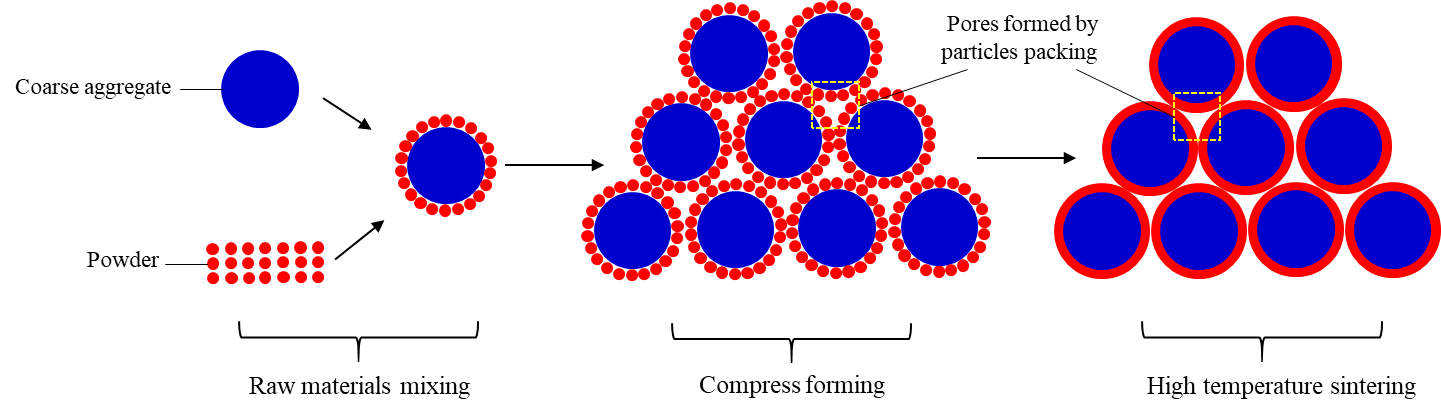
\includegraphics[width=1.0\textwidth]{Fig3-1.png}
    \bicaption{颗粒堆积型多孔材料制备过程和结构示意图}
    {Schematic diagram of the preparation process and structure of porous permeable brick generated by particle packing\\
    \textcolor{red}{(宋体、Times New Roman 5号字加粗,居中置于图的下方)}}
    \label{Fig3-1}
\end{figure}
\clearpage
多图
\begin{figure}[!htbp]
    \centering
    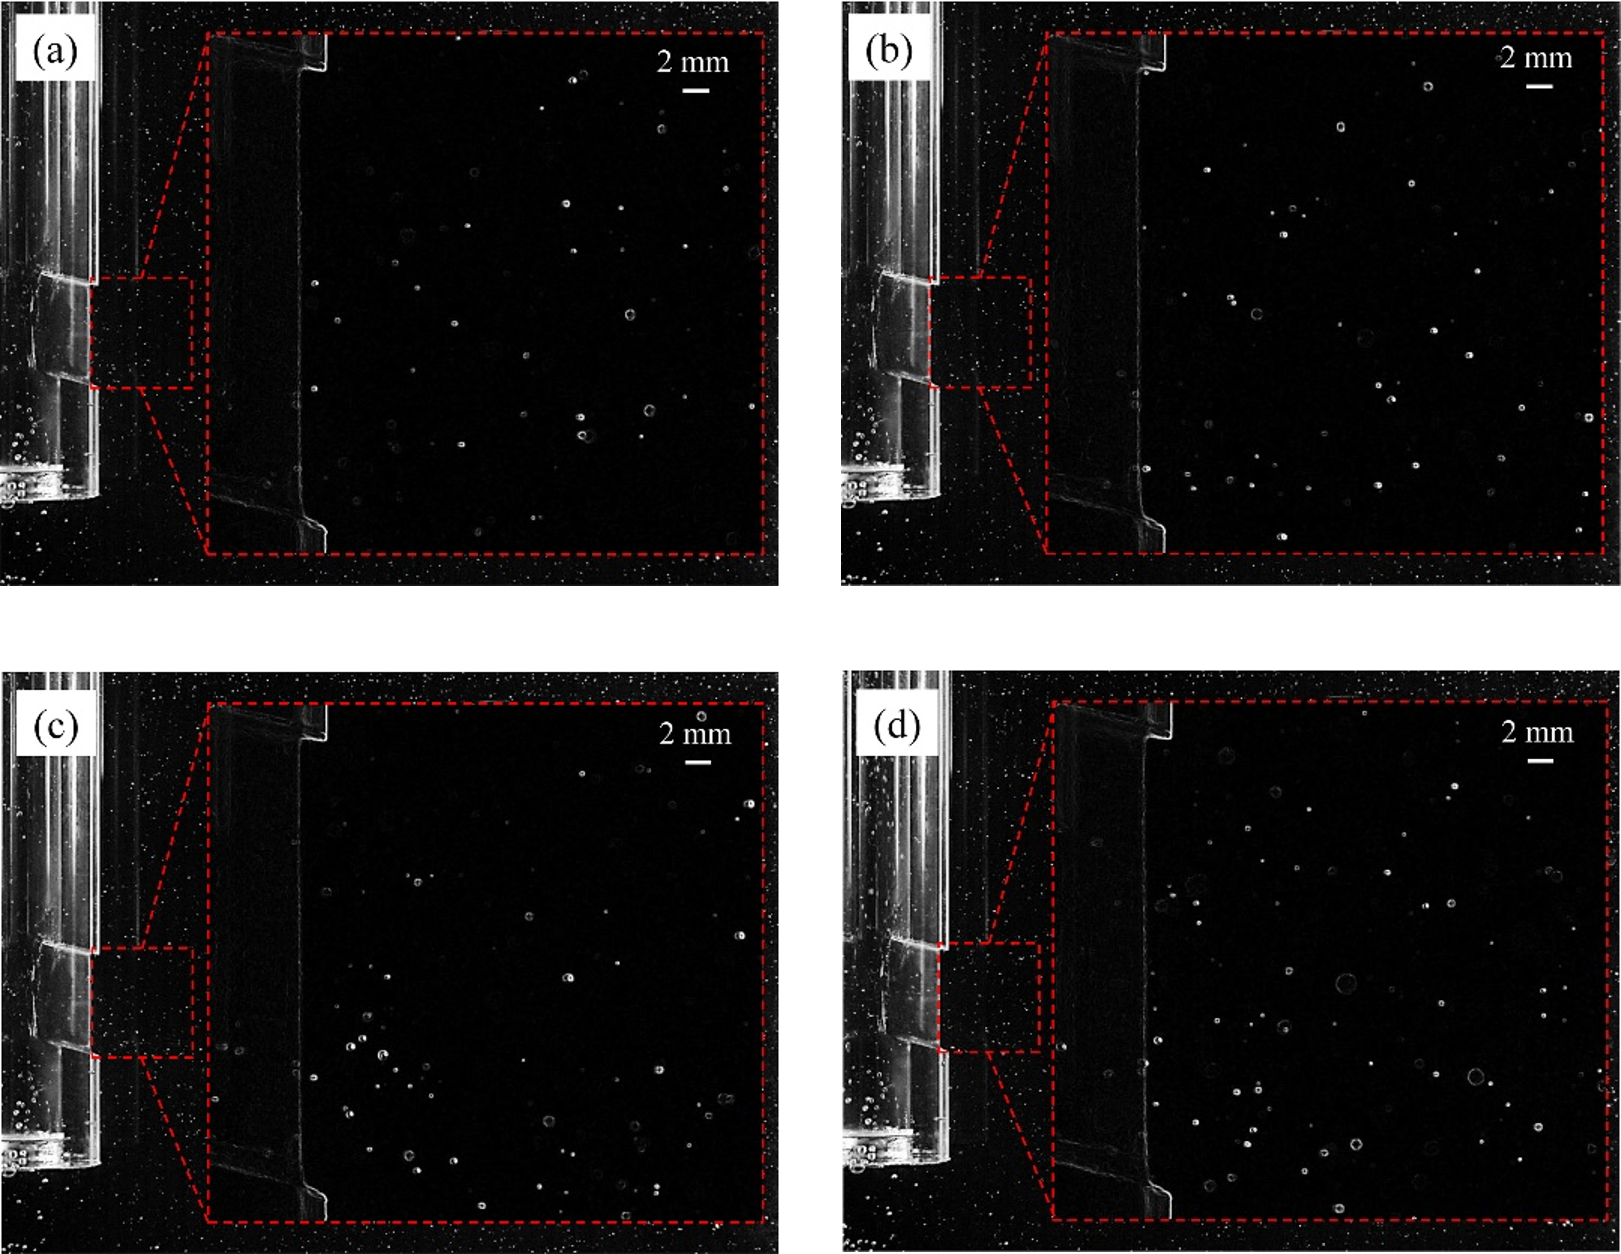
\includegraphics[width=1.0\textwidth]{Fig3-2.png}
    \bicaption{\boldmath 不同吹氩量下结晶器水模型内气泡形貌:(a)2 L·min$^{-1}$;(b)4 L·min$^{-1}$;(c)6 L·min$^{-1}$;(d)8 L·min$^{-1}$}
    {Bubble morphology in mold at different argon flow rates from water model experiment: (a) 2 L·min$^{-1}$; (b) 4 L·min$^{-1}$; (c) 6 L·min$^{-1}$; (d) 8 L·min$^{-1}$\\
    \textcolor{red}{(宋体、Times New Roman 5号字加粗,居中置于图的下方)}}
    \label{Fig3-1}
\end{figure}
\clearpage
\chapter[表的撰写规范]{表的撰写规范{\song\xiaosi \textcolor{red}{(黑体小二号加粗,段后1行,居中)}}}

\section[二级标题]{二级标题{\song\xiaosi \textcolor{red}{(黑体小三号字加粗,前后段间距0.5行,不空格)}}}

\subsection[三级标题]{三级标题{\song\xiaosi \textcolor{red}{(黑体四号字加粗,前后段间距0.25行,不空格)}}}
表中参数应标明量和单位的符号。

表按章编号,表序及表名置于表的上方,宋体五号字加粗,居中。

若表有附注,采用英文小写字母顺序编号,附注写在表的下方。 

表与正文之间要有一行的间距,如:
\begin{table}[!htbp]
    \centering
    \bicaption{\boldmath 1号试样渗透率测试数据(温度:T=16~$^\circ$C\quad 高度:H=5.31 mm)}{\boldmath Penetration rate of sample 1 (temperature: T=16~$^\circ$C\quad height: H=5.31 mm)}
    \resizebox{1.0\textwidth}{!}{
        \begin{tabular}{cccccc}
            \toprule[1.5pt]
            \makecell[c]{供气压力\\$Ps$ (MPa)}  & \makecell[c]{流量测量\\$M^\prime$ (m$^3$/h)}  & \makecell[c]{流量修正值\\$M$ (m$^3$/s)$\times 10^{-4}$}  & \makecell[c]{压力差\\$\varDelta P$ (Pa)}  & lg$\varDelta P$  & lg$M$    \\
            \midrule[0.75pt]   
            0.15                                & 0.009                                         & 0.02312                                                  & 46900                                     & 4.67117          & -5.63601  \\
            0.2	                                & 0.021                                         & 0.04584                                                  & 96900                                     & 4.98632          & -5.33876  \\                           
            0.25                                & 0.039                                         & 0.07413                                                  & 146900                                    & 5.16702          & -5.13001  \\ 
            0.3	                                & 0.097                                         & 0.16747                                                  & 196900                                    & 5.29424          & -4.77606  \\ 
            0.35                                & 0.136                                         & 0.21753                                                  & 246900                                    & 5.39252          & -4.66248  \\
            \bottomrule[1.5pt]   
      \end{tabular}
    }
      \label{tab4-1}
\end{table}

\textcolor{red}{表题宋体、Times New Roman 5号字加粗;表序与表题之间空一格置于表的上面,表格内容5号宋体不加粗;表格内指定高度设置为0.8 cm,行高值设置为最小值。表格如跨页需采用续表,如下:}
\begin{table}[!htbp]
    \centering
    \resizebox{1.0\textwidth}{!}{
        \begin{tabular}{cccccc}
            \toprule[1.5pt]
            \makecell[c]{供气压力\\$Ps$ (MPa)}  & \makecell[c]{流量测量\\$M^\prime$ (m$^3$/h)}  & \makecell[c]{流量修正值\\$M$ (m$^3$/s)$\times 10^{-4}$}  & \makecell[c]{压力差\\$\varDelta P$ (Pa)}  & lg$\varDelta P$  & lg$M$    \\
            \midrule[0.75pt]   
            0.15                                & 0.009                                         & 0.02312                                                  & 46900                                     & 4.67117          & -5.63601  \\
            0.2	                                & 0.021                                         & 0.04584                                                  & 96900                                     & 4.98632          & -5.33876  \\                           
            \bottomrule[1.5pt]   
      \end{tabular}
    }
      \label{tab4-1}
\end{table}

\include{body/chap05}

%%% 结论
\chapter[结论与展望]{结论与展望{\song\xiaosi \textcolor{red}{(黑体小二号加粗,段后1行,居中)}}}

结论是对整个论文主要成果的总结,在\textbf{结论中应明确指出本研究内容的创造性成果或创新点理论(含新见解、新观点)},
对其应用前景和社会、经济价值等加以预测和评价,并指出今后进一步在本研究方向进行研究工作的展望与设想。应准确、完整、明确和精练。

\section{参考文献示例}
\v{S}mejkal等人用群论描述交错磁性\cite{altermagnetic1,altermagnetic2},Zhang等人提出$\cdots\cdots$,详见文献\inlinecite{CrXO}和\inlinecite{OsO2}。

{\color{red}

    参考文献说明:
    
    (内容用宋体、Times New Roman,小四号,1.25倍行距)

[1]	[期刊文章] 作者(三人以内的全列出,超出3人的用“等”字代替). 文题[J]. 刊名,年,卷(期):起始页码-终止页码.

[2]	[专著] 作者. 书名[M]. 出版地:出版社,出版年:起始页码-终止页码

[3]	[译著] 作者. 书名[M]. 译者. 出版地:出版者,出版年.

[4]	[会议论文集] 编者. 文集[C]. 出版地:出版者,出版年. 起始页码-终止页码.

[5]	[析出文献] 作者. 析出文献题名[C]∥原文献主要责任者. 原文献题名:其他题名信息(如副标题). 出版地:出版者,出版年:析出文献起始页码-终止页码.

[6]	[学位论文] 作者. 文题[D]. 所在城市:保存单位,年份.

[7]	[专利] 申请者. 专利名: 国名,专利号[P].发布日期. 

[8]	[技术标准] 标准编号, 标准名称[S].

[9]	[技术报告] 作者. 文题[R]. 报告代码及编号,地名:责任单位,年份. 

[10]	[在线文献] 作者. 文题[EB/OL].(公告日期)[引用日期]. http://…, 日期.

[11]	[外文参考文献](英文参考文献中,作者姓名均姓前名后,姓写全称,名字缩写;论文题名首字母大写,其余小写,期刊名称每个单词首字母大写(介词和连词小写);杂志名要求写全称。)

[12]	已公开发表的文献不得用预印版链接格式引用
}


%%% 致谢

%%% Local Variables:
%%% mode: latex
%%% TeX-master: "../main"
%%% End:

\begin{ack}

致谢对象限于在学术方面对论文的完成有较重要帮助的团体和个人(300字左右)。包括内容如下:

(1)	对国家科学基金、资助研究工作的奖学金基金、合同单位、资助或支持的企业、组织或个人。

(2)	对协助完成研究工作和提供便利条件的组织或个人。

(3)	对在研究工作中提出建议和提供帮助的人。

(4)	对给予转载和引用权的资料、图片、文献、研究思想和设想的所有者。

(5)	对其他应感谢的组织和个人。

\textcolor{red}{(致谢应实事求是,切忌浮夸与庸俗之词。致谢正文使用标准字间距、宋体小四号字、1.25倍行距。)}
\end{ack}



%%% 参考文献
%Included for Gather Purpose only:
%input "ref/refs.bib"
\bibliographystyle{WUSTThesis}
\bibliography{./ref/refs}

%%% 附录(根据自己实际情况增加或删减)
\begin{appendix}
%\chapter{答辩委员会决议}
首行缩进两个字符,中文字体采用小四宋体,英文字体采用Times New Roman,字体大小为小四,行间距为固定值20磅。
%% 根据自己实际情况增加或删减
\begin{publications}
\noindent
\renewcommand{\labelenumi}{[\arabic{enumi}]}
\begin{spacing}{1.25}
\begin{enumerate}
\item \textbf{Wancheng Zhang}, Mingkun Zheng, Yong Liu, Zhenhua Zhang, Rui Xiong, and Zhihong Lu. Strain-induced nonrelativistic altermagnetic spin splitting effect[J]. Physical Review B, 2025, 112, 024415.
\item \textbf{Wancheng Zhang}, Mingkun Zheng, Yong Liu, Pan Zhang, Zhenhua Zhang, Rui Xiong, and Zhihong Lu. Unconventional spin Hall effect in rutile ${\mathrm{Cr}}_{0.5}{X}_{0.5}{\mathrm{O}}_{2}$ $(X=\mathrm{Ti},\mathrm{V},\mathrm{Os},\mathrm{Fe})$[J]. Physical Review B, 2024, 110(21), 214419.
\item \textbf{Wancheng Zhang}, Mingkun Zheng, Yong Liu, Rui Xiong, Chao Zuo, Meng Chen, Zhenhua Zhang, and Zhihong Lu. Oxygen-vacancy-mediated efficient charge-to-spin conversion in heavy-metal oxides[J]. Journal of Physics D: Applied Physics. (Under review).
\item Mingkun Zheng, \textbf{Wancheng Zhang}, You Lv, Yong Liu, Rui Xiong, Zhenhua Zhang, and Zhihong Lu. Observation of thickness-modulated out-of-plane spin-orbit torque in polycrystalline few-layer $T_d$-\ce{WTe2} film[J]. Nanomaterials, 2025, 15(10), 762.
\item Mingkun Zheng, \textbf{Wancheng Zhang}, You Lv, Yong Liu, Rui Xiong, Zhenhua Zhang, and Zhihong Lu. Low-temperature fabrication, magnetoresistance and spin pumping studies of polycrystalline few-layer 1$T$'-\ce{MoTe2} films. Journal of Alloys and Compounds, 2025, 1015, 178775.
\item Jindi Feng, \textbf{Wancheng Zhang}, Kunpeng Li, Mingkun Zheng, Yong Liu, Chao Zuo, Meng Chen, Dengjing Wang, Youyuan Yuan, Ke Wang, Zhenhua Zhang, Rui Xiong, and Zhihong Lu. Tailoring of band alignments and magnetic properties in two-dimensional \ce{CrBr3}/\ce{MoS2} van der Waals heterobilayer. Computational Materials Science, 2024, 236, 112862.
\item Kunpeng Li, Jindi Feng, \textbf{Wancheng Zhang}, Zhenhua Zhang, Rui Xiong, and Zhihong Lu. Enhancing spin splitting by symmetry and molecular orbital hybridization in \ce{VO2}. Computational Materials Science, 2023, 222, 112100.
\item Jindi Feng, Kunpeng Li, Mingkun Zheng, \textbf{Wancheng Zhang}, Yong Liu, Dengjing Wang, Zhenhua Zhang, Chao Zuo, Rui Xiong, and Zhihong Lu. Excellent spin-filtering and giant tunneling magnetoresistance in a dual-electrode van der Waals magnetic tunnel junction based on ferromagnetic \ce{CrSe2}. Applied Surface Science, 2023, 611, 155588.
\end{enumerate}
\end{spacing}
\end{publications}

%\chapter{公开发表的学术论文与博士学位论文的关系}
\begin{center} 
\song \xiaosi
%\vspace{2.0cm}
\renewcommand{\arraystretch}{1.5}
\begin{longtable}{|p{0.9cm}<{\centering}|p{2.8cm}<{\centering}|p{2.4cm}<{\centering}|p{3cm}<{\centering}|p{4cm}<{\centering}|}
    \hline
    \makecell{序号}&\makecell[c]{成果名称}&\makecell[c]{成果形式}&\makecell[c]{成果主要内容}&\makecell[c]{与学位论文对应的关系}\\
    \hline
    1&\makecell[c]{}
    & \makecell[c]{}
    & \makecell[c]{}
    & \makecell[c]{}\\
    \hline
    2&\makecell[c]{}
    & \makecell[c]{}
    & \makecell[c]{}
    & \makecell[c]{}\\
    \hline
    3&\makecell[c]{}
    & \makecell[c]{}
    & \makecell[c]{}
    & \makecell[c]{}\\
    \hline
    4&\makecell[c]{}
    & \makecell[c]{}
    & \makecell[c]{}
    & \makecell[c]{}\\
    \hline
    5&\makecell[c]{}
    & \makecell[c]{}
    & \makecell[c]{}
    & \makecell[c]{}\\
    \hline
\end{longtable}
\end{center}  

%\chapter{攻读博士学位期间参与的科研项目}
\begin{project}
\renewcommand{\labelenumi}{[\arabic{enumi}]}
\begin{spacing}{1.25}
   \begin{enumerate}
    \item 反铁磁\ce{FePt_{1-x}Rh_x}薄膜中的各向异性电输运特性, 国家自然科学基金, 项目编号:12204364 (参与)
    \item 半金属氧化物\ce{CrO2}薄膜的磁阻尼调控及机理, 国家自然科学基金, 项目编号:12204364 (参与)
   \end{enumerate}
\end{spacing}
\end{project} 

%\chapter{中英文缩写对照表}
\begin{center} \xiaosi
%\vspace{2.0cm}
\renewcommand{\arraystretch}{1.5}
\begin{tabular}{p{2.3cm}p{12.7cm}}
    3D&Three-dimensional(三维)\\
    CT&Computer tomography (计算机断层层析成像)\\
    MRI&Magnetic resonance imaging(磁共振成像)\\
    PET&Positron emission computed tomography(正电子发射断层成像)\\
    …&
\end{tabular}
\end{center}  
%\chapter{其它数据图表或程序}
\end{appendix}
\end{sloppypar}
\end{document}
